\documentclass[bluish,slideColor,colorBG,pdf]{prosper}
\hypersetup{pdfpagemode=FullScreen}
\usepackage{graphicx,amsfonts,amsmath,color,bm}
\def\baselinestretch{1.0}
\setlength{\topmargin}{-60pt}
\setlength{\textheight}{460pt}
\setlength{\oddsidemargin}{0pt}
\setlength{\evensidemargin}{0pt}
\setlength{\textwidth}{660pt}
\setlength{\footskip}{0pt}
\parindent 0.3in
\hyphenpenalty=10000
\tolerance=10000
\pagestyle{empty}

\def\Prob{{\rm Prob\;}}
\def\prob{{\rm \;Prob\;}}
\def\PROB{{\rm \;Prob}}
\def\Var{{\rm Var}}        % Var
\def\Cov{{\rm Cov}}        % Cov

\DeclareSymbolFont{AMSb}{U}{msb}{m}{n}
\DeclareMathSymbol{\expect}{\mathalpha}{AMSb}{'105}

\title{Week 4:  Consistency; History / philosophy, distance methods}
\author{Genome 570}
\institution{January, 2016}

\definecolor{golden}{rgb}{1.0,0.8,0.3}
\definecolor{gold}{rgb}{0.9,0.6,0.3}
\definecolor{purple}{rgb}{1.0,0,1.0}
\definecolor{red}{rgb}{1.0,0.0,0}

\begin{document}

\maketitle

\begin{slide}[Replace]{The counterexample}

\centerline{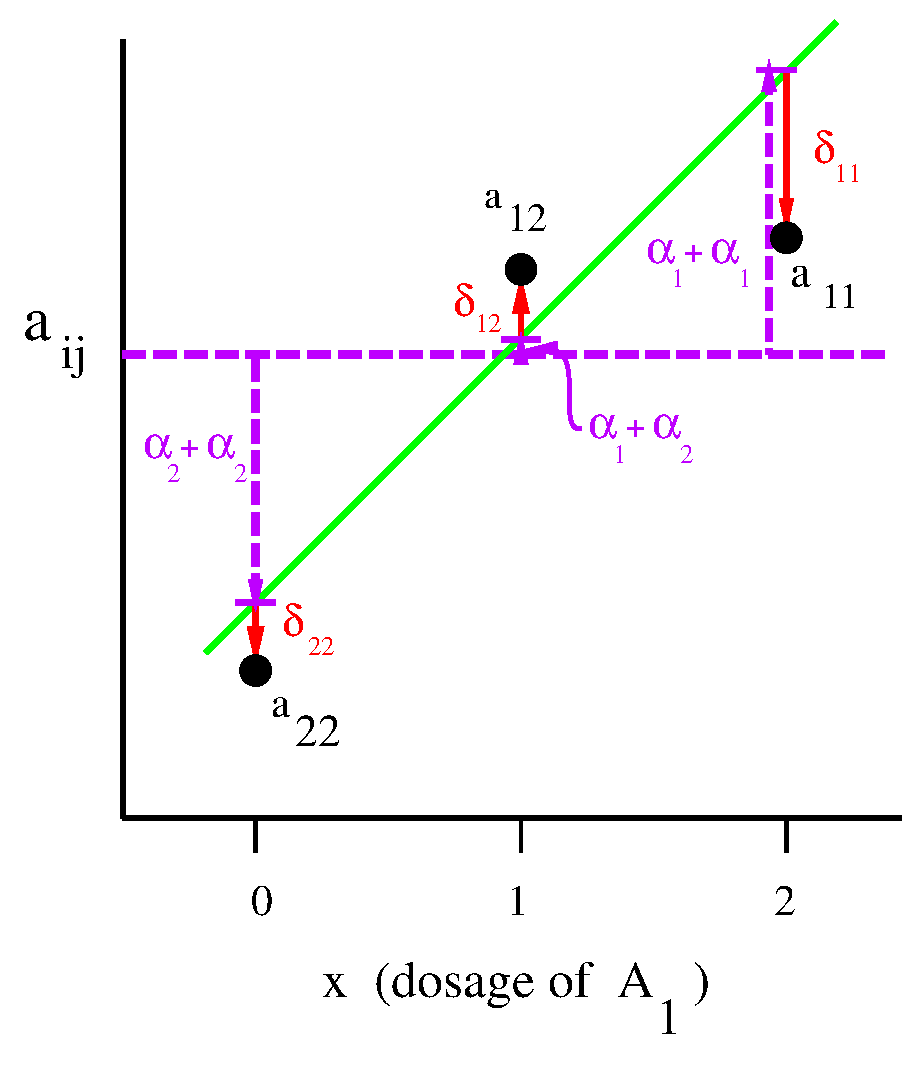
\includegraphics[width=2.5in]{fig9-3.ydraw}}
\bigskip

The long branches have probabilities of change $\ \mathsf{p}$, the short
branches have probabilities of change $\ \mathsf{q}$.  This is the canonical
case of ``long branch attraction''.

\end{slide}

\begin{slide}[Replace]{Pattern probabilities}

If tip pattern is 1100, and internal nodes are 1, 1 the probability is
\[
\mathsf{\frac{1}{2}(1-p)(1-q)(1-q)pq}
\]

and in general summing over all four possibilities:
\[
\begin{array}{c c l}
\mathsf{P_{1100}} & \mathsf{=} &  \mathsf{\frac{1}{2}\left((1-p)(1-q)^2pq\ +\ (1-p)^2(1-q)^2q\right.}\\
& & \\
  & & \mathsf{\left.+\ p^2q^3\ +\ pq(1-p)(1-q)^2\right)}
\end{array}
\]

\end{slide}

\begin{slide}[Replace]{Pattern probabilities}

\noindent
\[
\begin{array}{c c l}
\mathsf{P_{xxyy}} &  \mathsf{=} &  \mathsf{(1-p)(1-q)[q(1-q)(1-p)\ +\ q(1-q)p]}\\\
& & \\
& &  \mathsf{+\  pq[(1-q)^2(1-p)\ +\ q^2p]} \\
& & \\
& & \\
\mathsf{P_{xyxy}} & \mathsf{=} & \mathsf{(1-p)q[q(1-q)p+q(1-q)(1-p)]}\\
& & \\
 & & \mathsf{+\ p(1-q)[p(1-q)^2\ +\ (1-p)q^2]} \\
& & \\
& & \\
\mathsf{P_{xyyx}} & \mathsf{=} &  \mathsf{(1-p)q[(1-p)q^2+p(1-q)^2]}\\
& & \\
 & &\mathsf{+\ p(1-q)[q(1-q)p +\ q(1-q)(1-p)]}
\end{array}
\]
 
\end{slide}

\begin{slide}[Replace]{Taking differences}

\noindent
\[
\mathsf{P_{xyxy} - P_{xyyx} \ =\ (1-2q)\;\left[q^2(1-p)^2\ +\ (1-q)^2p^2\right]}
\]
\medskip

Which is always positive as long as $\mathsf{~q < 1/2~}$ and either
$\mathsf{~p~}$ or $\mathsf{~q~}$ is positive.  Thus $\mathsf{~P_{xyxy} >
P_{xyyx}~}$ so we don't need to concern ourselves with $\ \mathsf{P_{xyyx}}$.
\bigskip

To have $\mathsf{P_{xxyy}}$ be the largest of the three, we only need to
know that
\[
\mathsf{P_{xxyy} - P_{xyxy}\ >\ 0}
\]

and after a struggle that turns out to require
\[
\mathsf{(1-2q)\;\left[q(1-q)\ -\ p^2 \right]\ >\ 0}
\]

which (provided $\mathsf{q < 1/2}$) is true if and only if
\[
\mathsf{q(1-q)\  >\  p^2}
\]

\end{slide}

\begin{slide}[Replace]{Pattern frequencies win out}
\bigskip

\centerline{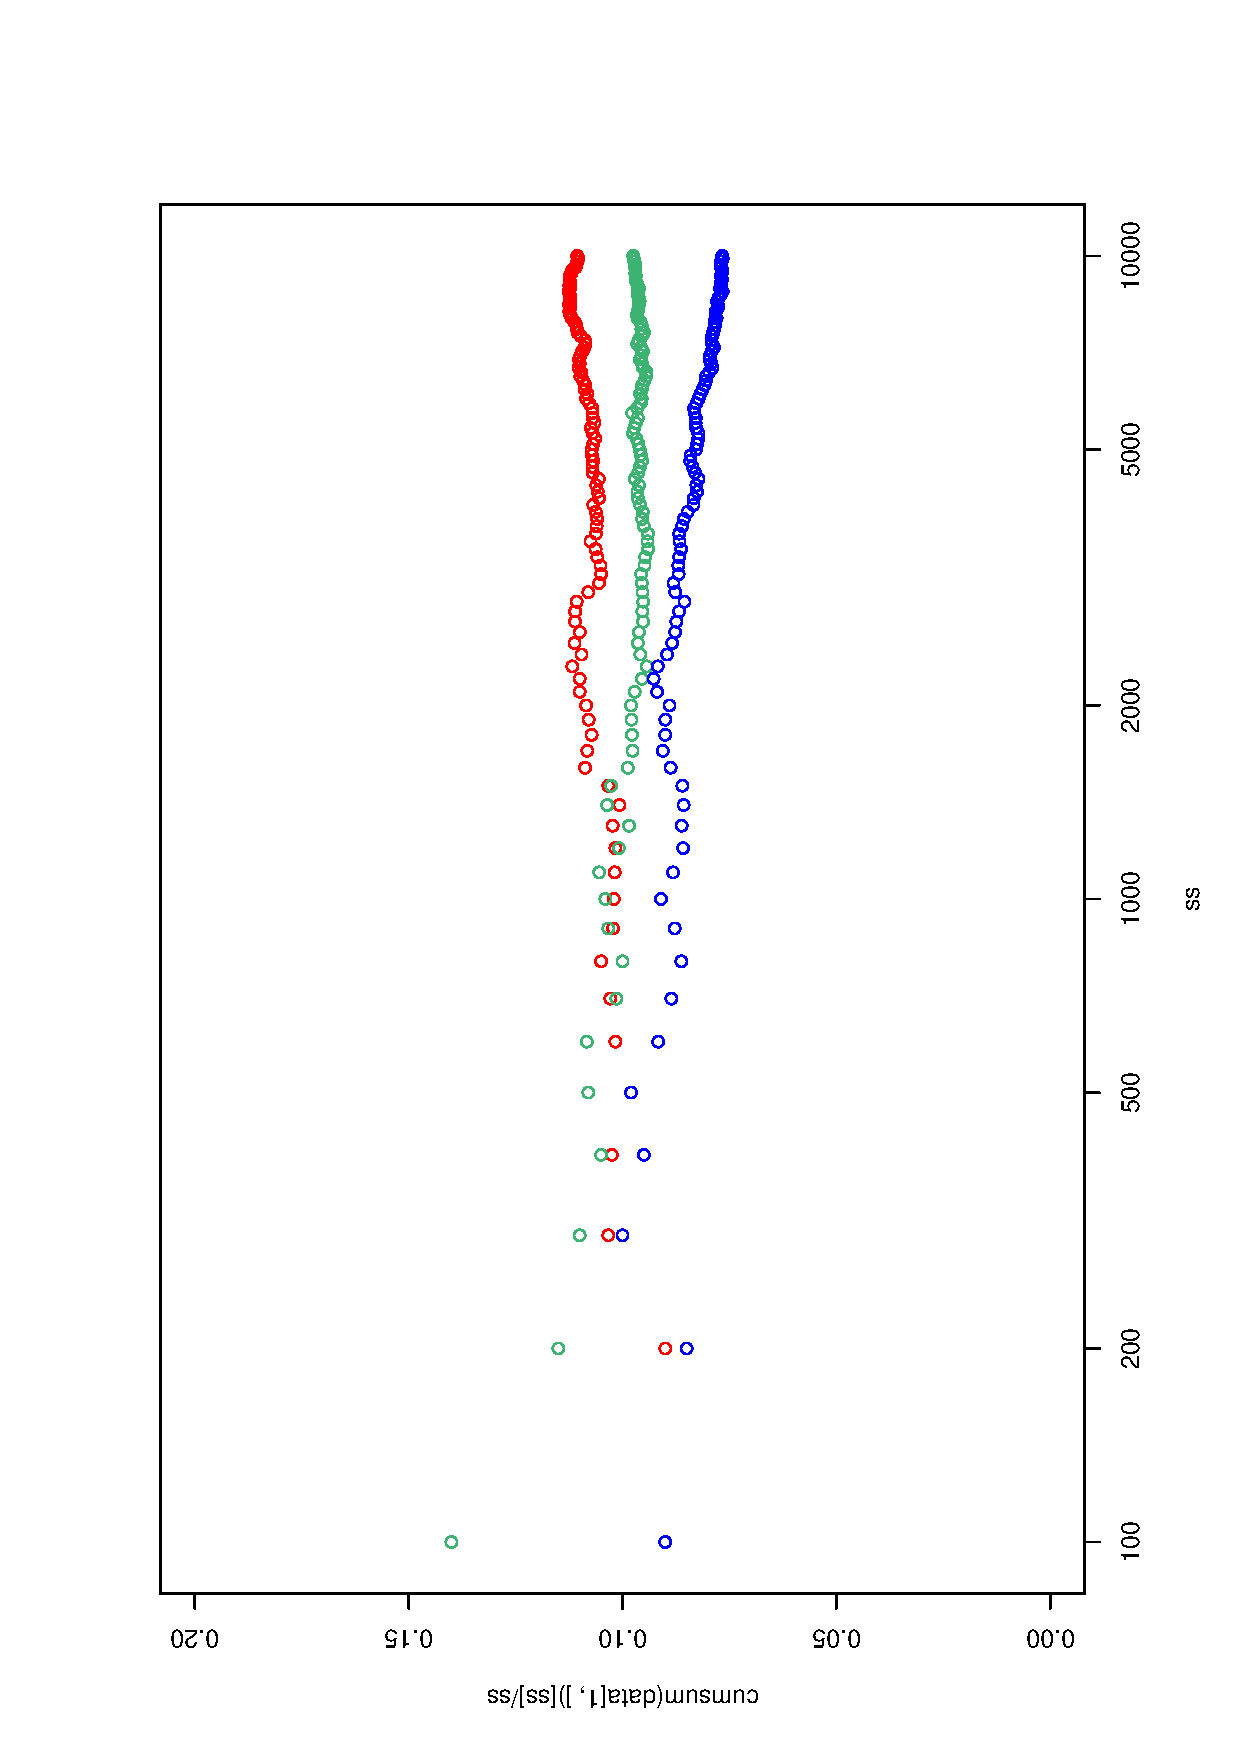
\includegraphics[width=4.0in]{largenumbers.idraw}}

\end{slide}

\begin{slide}[Replace]{Conditions for inconsistency}

\centerline{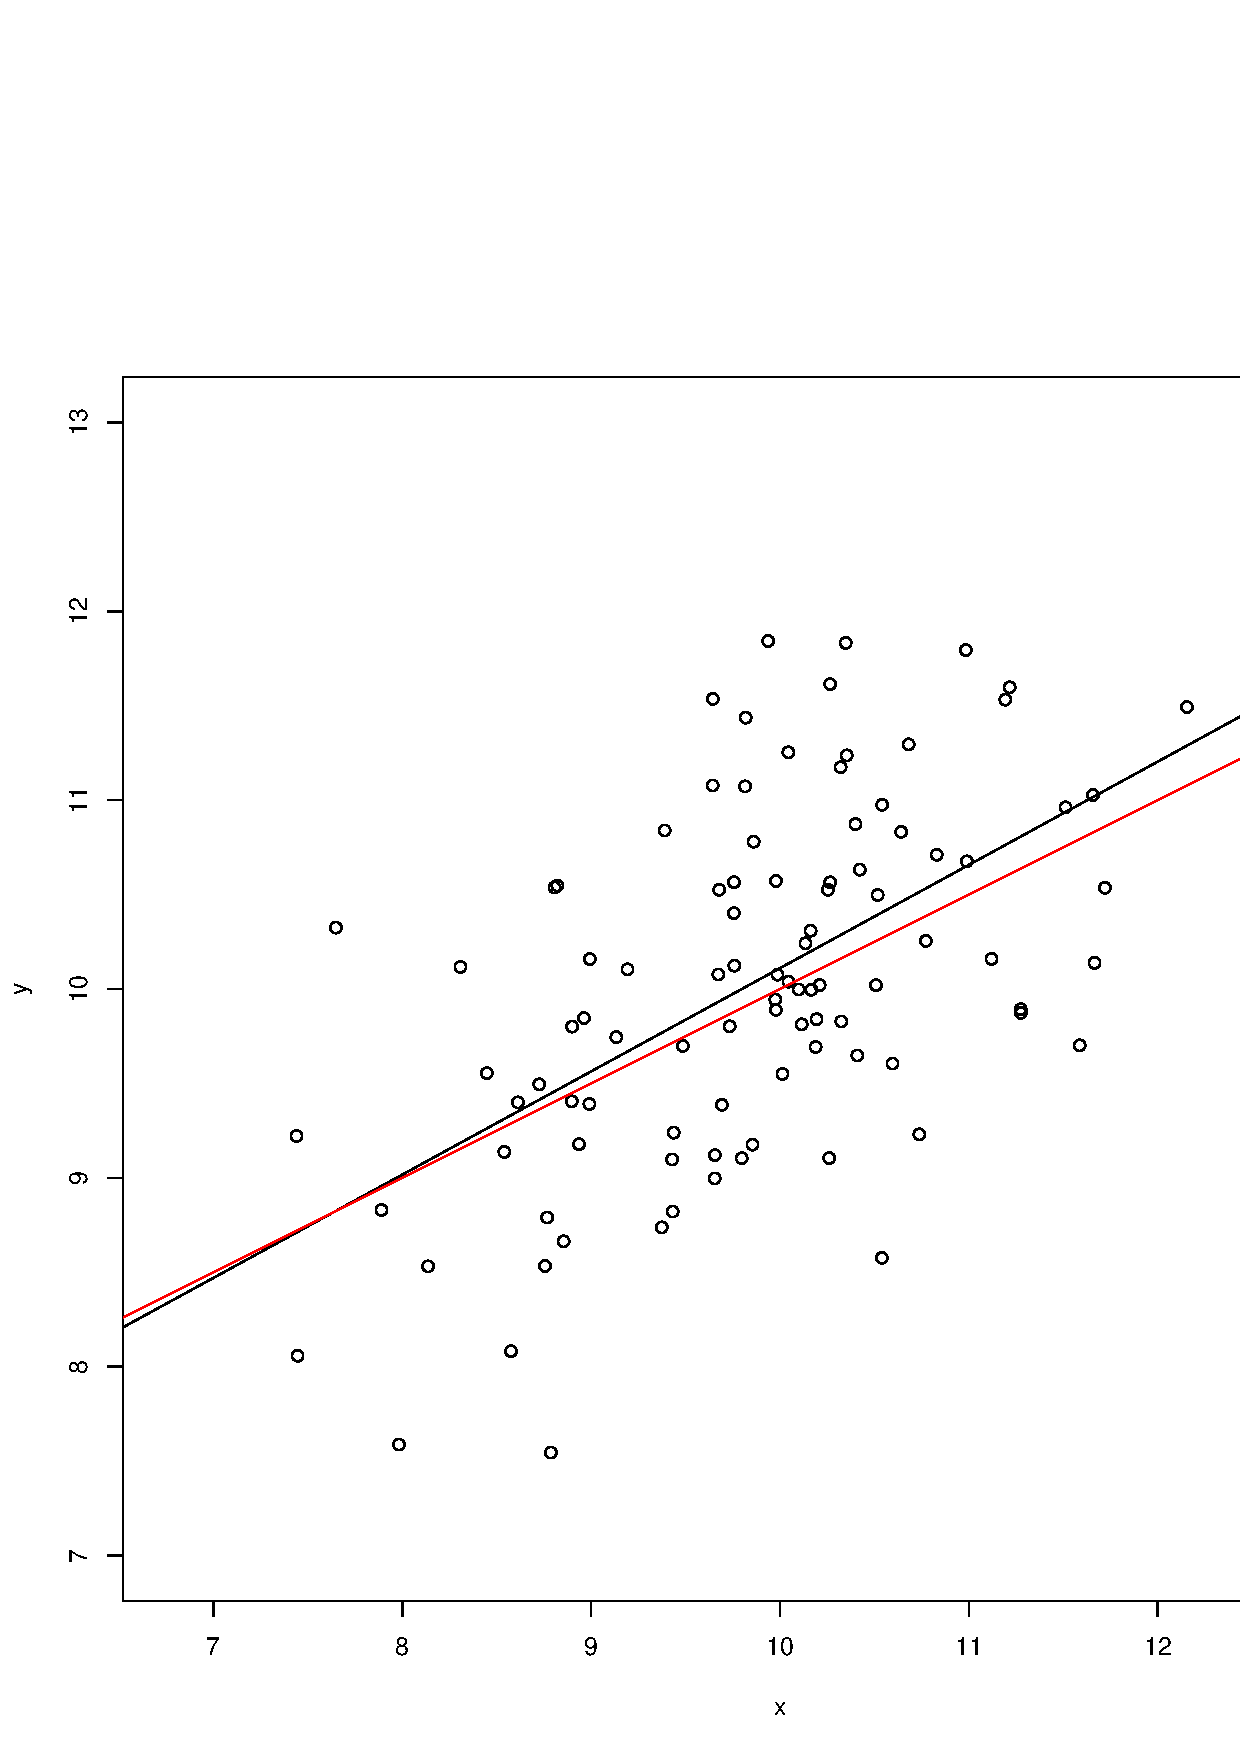
\includegraphics[width=3.2in]{fig9-5.ydraw}}

\end{slide}

\begin{slide}[Replace]{Example for patterns with DNA}

\centerline{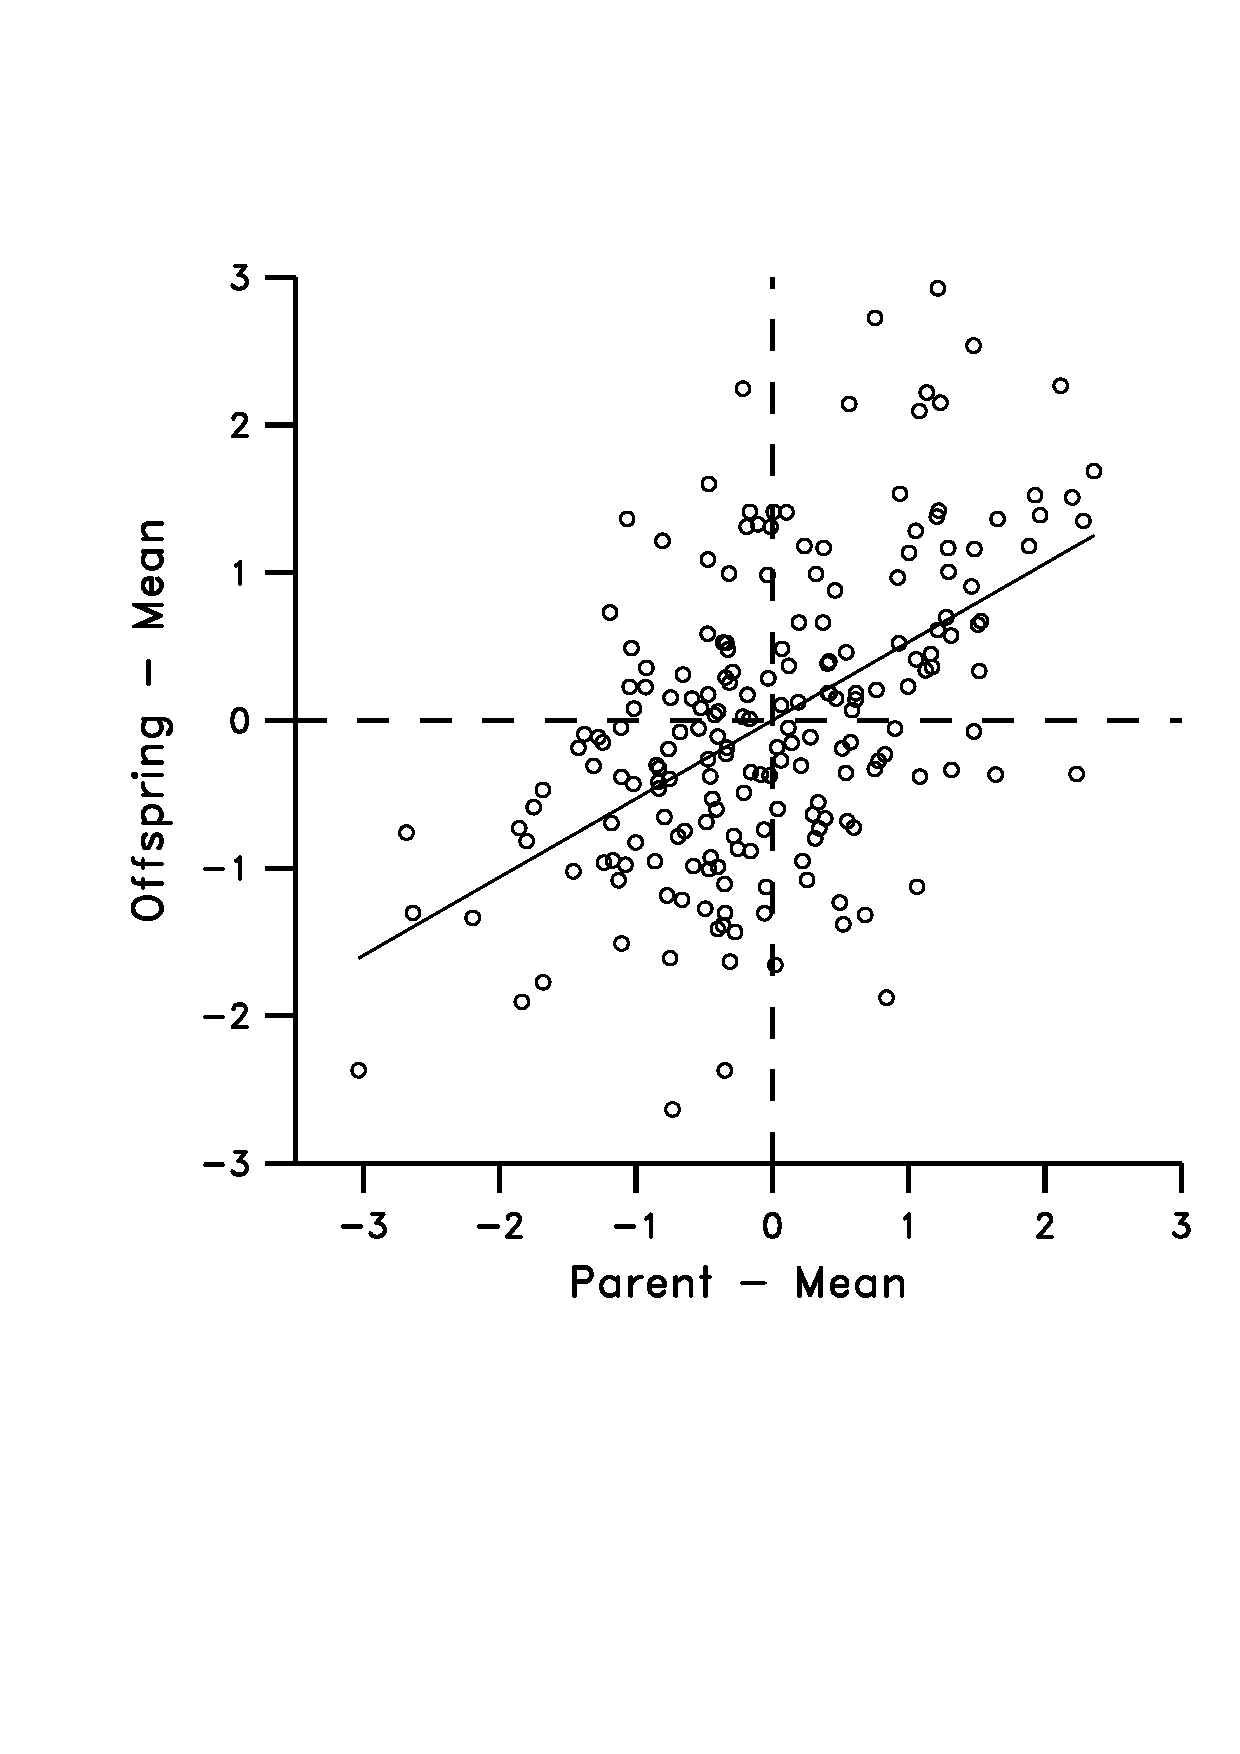
\includegraphics[width=2.5in]{fig9-6.ydraw}}

\end{slide}

\begin{slide}[Replace]{Calculating a pattern frequency}

\noindent
\[
\begin{array}{c c l}
\mathsf{\prob[CCAA]} & \mathsf{=} & \mathsf{\frac{1}{18}\,(1-p)(1-q)^2pq\ +\ \frac{1}{27}\,pq^2(1-p)(1-q)}\\
& & \\
& & \mathsf{+\ \frac{1}{162}\,p^2q^2(1-q)\ +\ \frac{7}{972}\,p^2q^3\ }\\
& & \\
& & \mathsf{+\ \frac{1}{12}\,(1-p)^2(1-q)^2q}.
\end{array}
\]

\end{slide}

\begin{slide}[Replace]{Pattern frequencies}

\noindent
\[
\renewcommand{\arraystretch}{1.5}
\begin{array}{c c l}
\mathsf{\prob[xxyy]} &  \mathsf{=} & \mathsf{(1-p)^2q(1-q)^2\ +\ \frac{2}{3}\,p(1-p)q(1-q)^2}\\
& &  \mathsf{+\ \frac{4}{9}\,p(1-p)q^2(1-q)\ +\ \frac{2}{27}\,p^2q^2(1-q)}\\
& &  \mathsf{+\ \frac{7}{81}\,p^2q^3}\\
& & \\
\mathsf{\prob[xyxy]} &  \mathsf{=} & \mathsf{\frac{1}{3}\,(1-p)^2q^2(1-q)\ +\ \frac{2}{9}\,p(1-p)q^2(1-q)}\\
& & \mathsf{+\ \frac{4}{27}\,p(1-p)q^3\ +\ \frac{1}{3}\,p^2(1-q)^3\ } \\
& & \mathsf{+\ \frac{2}{9}\,p^2q^2(1-q)\ +\ \frac{2}{81}\,p^2q^3}\\
& & \\
\mathsf{\prob[xyyx]} & \mathsf{=} &  \mathsf{\frac{1}{81}\,(1-p)^2q^3\ +\ \frac{2}{3}\,p(1-p)q(1-q)^2}\\
& & \mathsf{+\ \frac{4}{9}\,p(1-p)q^3\ +\ \frac{1}{9}\,p^2q(1-q)^2}\\
& & \mathsf{+\ \frac{6}{27}\,p^2q^2(1-q)\ +\ \frac{2}{81}\,p^2q^3}.
\end{array}
\]

\end{slide}

\begin{slide}[Replace]{Conditions for inconsistency with DNA}
{~~}
\vfill

\noindent
\[
\mathsf{\frac{p\ <\ {{-18\,q + 24\,{q^2} + {\sqrt{243\,q - 567\,{q^2} + 648\,{q^3} -
288\,{q^4}}}}}{{9 - 24\,q + 32\,{q^2}}}}}
\]
\bigskip

(This will {\it not} be on the test).
\bigskip

For small $\mathsf{~p~}$ and $\mathsf{~q~}$ this is approximately
\[
\mathsf{\frac{1}{3}\,p^2 \ \ < \ \ q}
\]

\vfill

\vfill

\end{slide}

\begin{slide}[Replace]{Conditions for inconsistency with DNA}

\centerline{\includegraphics[width=3.0in]{fig9-7.ydraw}}

\end{slide}

\begin{slide}[Replace]{Inconsistency with a clock}

\centerline{\includegraphics[width=4in]{fig9-8.ydraw}}
\bigskip

Cases like this were discovered by Michael Hendy and David Penny in 1989.

\end{slide}
 
\begin{slide}[Replace]{Example showing inconsistency with a clock}

\centerline{\includegraphics[width=4in]{fig9-9.ydraw}}

\end{slide}

\begin{slide}[Replace]{History and philosophy}
\bigskip

Issues:
\begin{itemize}
\item How did work on numerical methods for phylogenies get started?
\item What is the logical basis of inferring phylogenies?
\item How does all that relate to classification?
\end{itemize}

\end{slide}

\begin{slide}[Replace]{Ernst Mayr and George Gaylord Simpson}
\vspace{-0.1in}

\centerline{\includegraphics[width=1.2in]{mayr1953.ps} \hspace{0.4in} \includegraphics[width=1.5in]{simpson.ps}}
\medskip

\centerline{\hspace*{0in}\hspace{0.2in}Ernst Mayr (1905-2005) \hspace{0.2in} George Gaylord Simpson (1902-1984)}

\begin{itemize}
\item Major figures in the completion of the ``modern synthesis'' or
``Neodarwinian
synthesis'' in the 1940s.
\item Leaders of the ``evolutionary systematics''
approach to taxonomic classification, dominant until the 1970s.
\end{itemize} 

\end{slide}

\begin{slide}[Replace]{Evolutionary-systematic classification}
\bigskip

\centerline{\includegraphics[height=2.3in]{mayrsimpson.idraw}}
\bigskip


A pattern of grades with very unequal rates of overall evolution is implicit
in the use of paraphyletic groups in Mayr and Simpson's practice.

\end{slide}

\begin{slide}[Replace]{A horse tree drawn by Simpson}
\vspace{-0.1in}

\centerline{\includegraphics[width=1.7in]{horses.ps}}
\medskip

Note the ``fat'' branches which are somewhat ambiguous.  As they emphasize
classification over phylogeny, are the trees starting to
dissolve?

\end{slide}

\begin{slide}[Replace]{A phylogeny of the living chordates}

\centerline{\includegraphics[width=3.0in]{chordates.ydraw}}
\medskip

... as an example of groups that are in the traditional classification system
but may or may not be monophyletic.

\end{slide}

\begin{slide}[Replace]{Vertebrates are a monophyletic group}

\centerline{\includegraphics[width=3.0in]{vertebrates.ydraw}}

\end{slide}

\begin{slide}[Replace]{Reptiles and fishes are paraphyletic groups}

\centerline{\includegraphics[width=3.0in]{paraphyletic.ydraw}}
\medskip

... since their most recent common ancestor is ancestral to other forms too
(such as us).

\end{slide}

\begin{slide}[Replace]{Positions on classification as of about 1960}

\begin{itemize}
\item \textcolor{purple}{Evolutionary systematics.} ~ George Gaylord Simpson and Ernst Mayr
led a movement that allowed non-monophyletic (paraphyletic) groups such
as reptiles, on the assumption that groups could be separated by real
differences of rates of evolution (sometimes ``grades'' rather than ``clades''). 
\item \textcolor{purple}{Phylogenetic systematics.} ~ Willi Hennig advocated purely monophyletic
classification.
\item \textcolor{purple}{Phenetics.} ~ Sokal and Sneath advocated making a classification without
reference to evolution, using numerical clustering methods
\end{itemize}

\end{slide}

\begin{slide}[Replace]{Technological change post World War II}
\bigskip

\begin{itemize}
\item Former physicists found molecular biology (first protein sequence, 1951)
\item Former codebreakers and atomic bomb builders build the early
computers (first stored-program digital computer, 1949)
\item Most U.S. universities got their first computer about 1957.
\item First sequences of same gene in multiple species in late 1950s.
\end{itemize}



\end{slide}

\begin{slide}[Replace]{Molecular evolution gets off the ground}

Zuckerkandl and Pauling in 1962 discussed using trees to infer ancestral
sequences, and named this ``chemical paleogenetics".  They were about
30 years ahead of their time.

\begin{center}
\begin{tabular}{c c}
{
\includegraphics[height=1.3in]{Zuckerkandl1986.ps}} &
{\includegraphics[height=1.3in]{pauling.ps}} \\
\parbox[t]{1.5in}{Emile Zuckerkandl\\in 1986} &
\parbox[t]{2.0in}{Linus in 1962, {\it from\\ Nobel Peace Prize web page}} \\
\end{tabular}
\end{center}
\medskip

(But then it isn't fair to anyone to compare them unfavorably to Linus
Pauling).

\end{slide}

\begin{slide}[Replace]{Peter Sneath in 1962 and Robert Sokal in 1964}

\begin{center}
\begin{tabular}{r l}
\includegraphics[height=1.9in]{sneath.ps} &
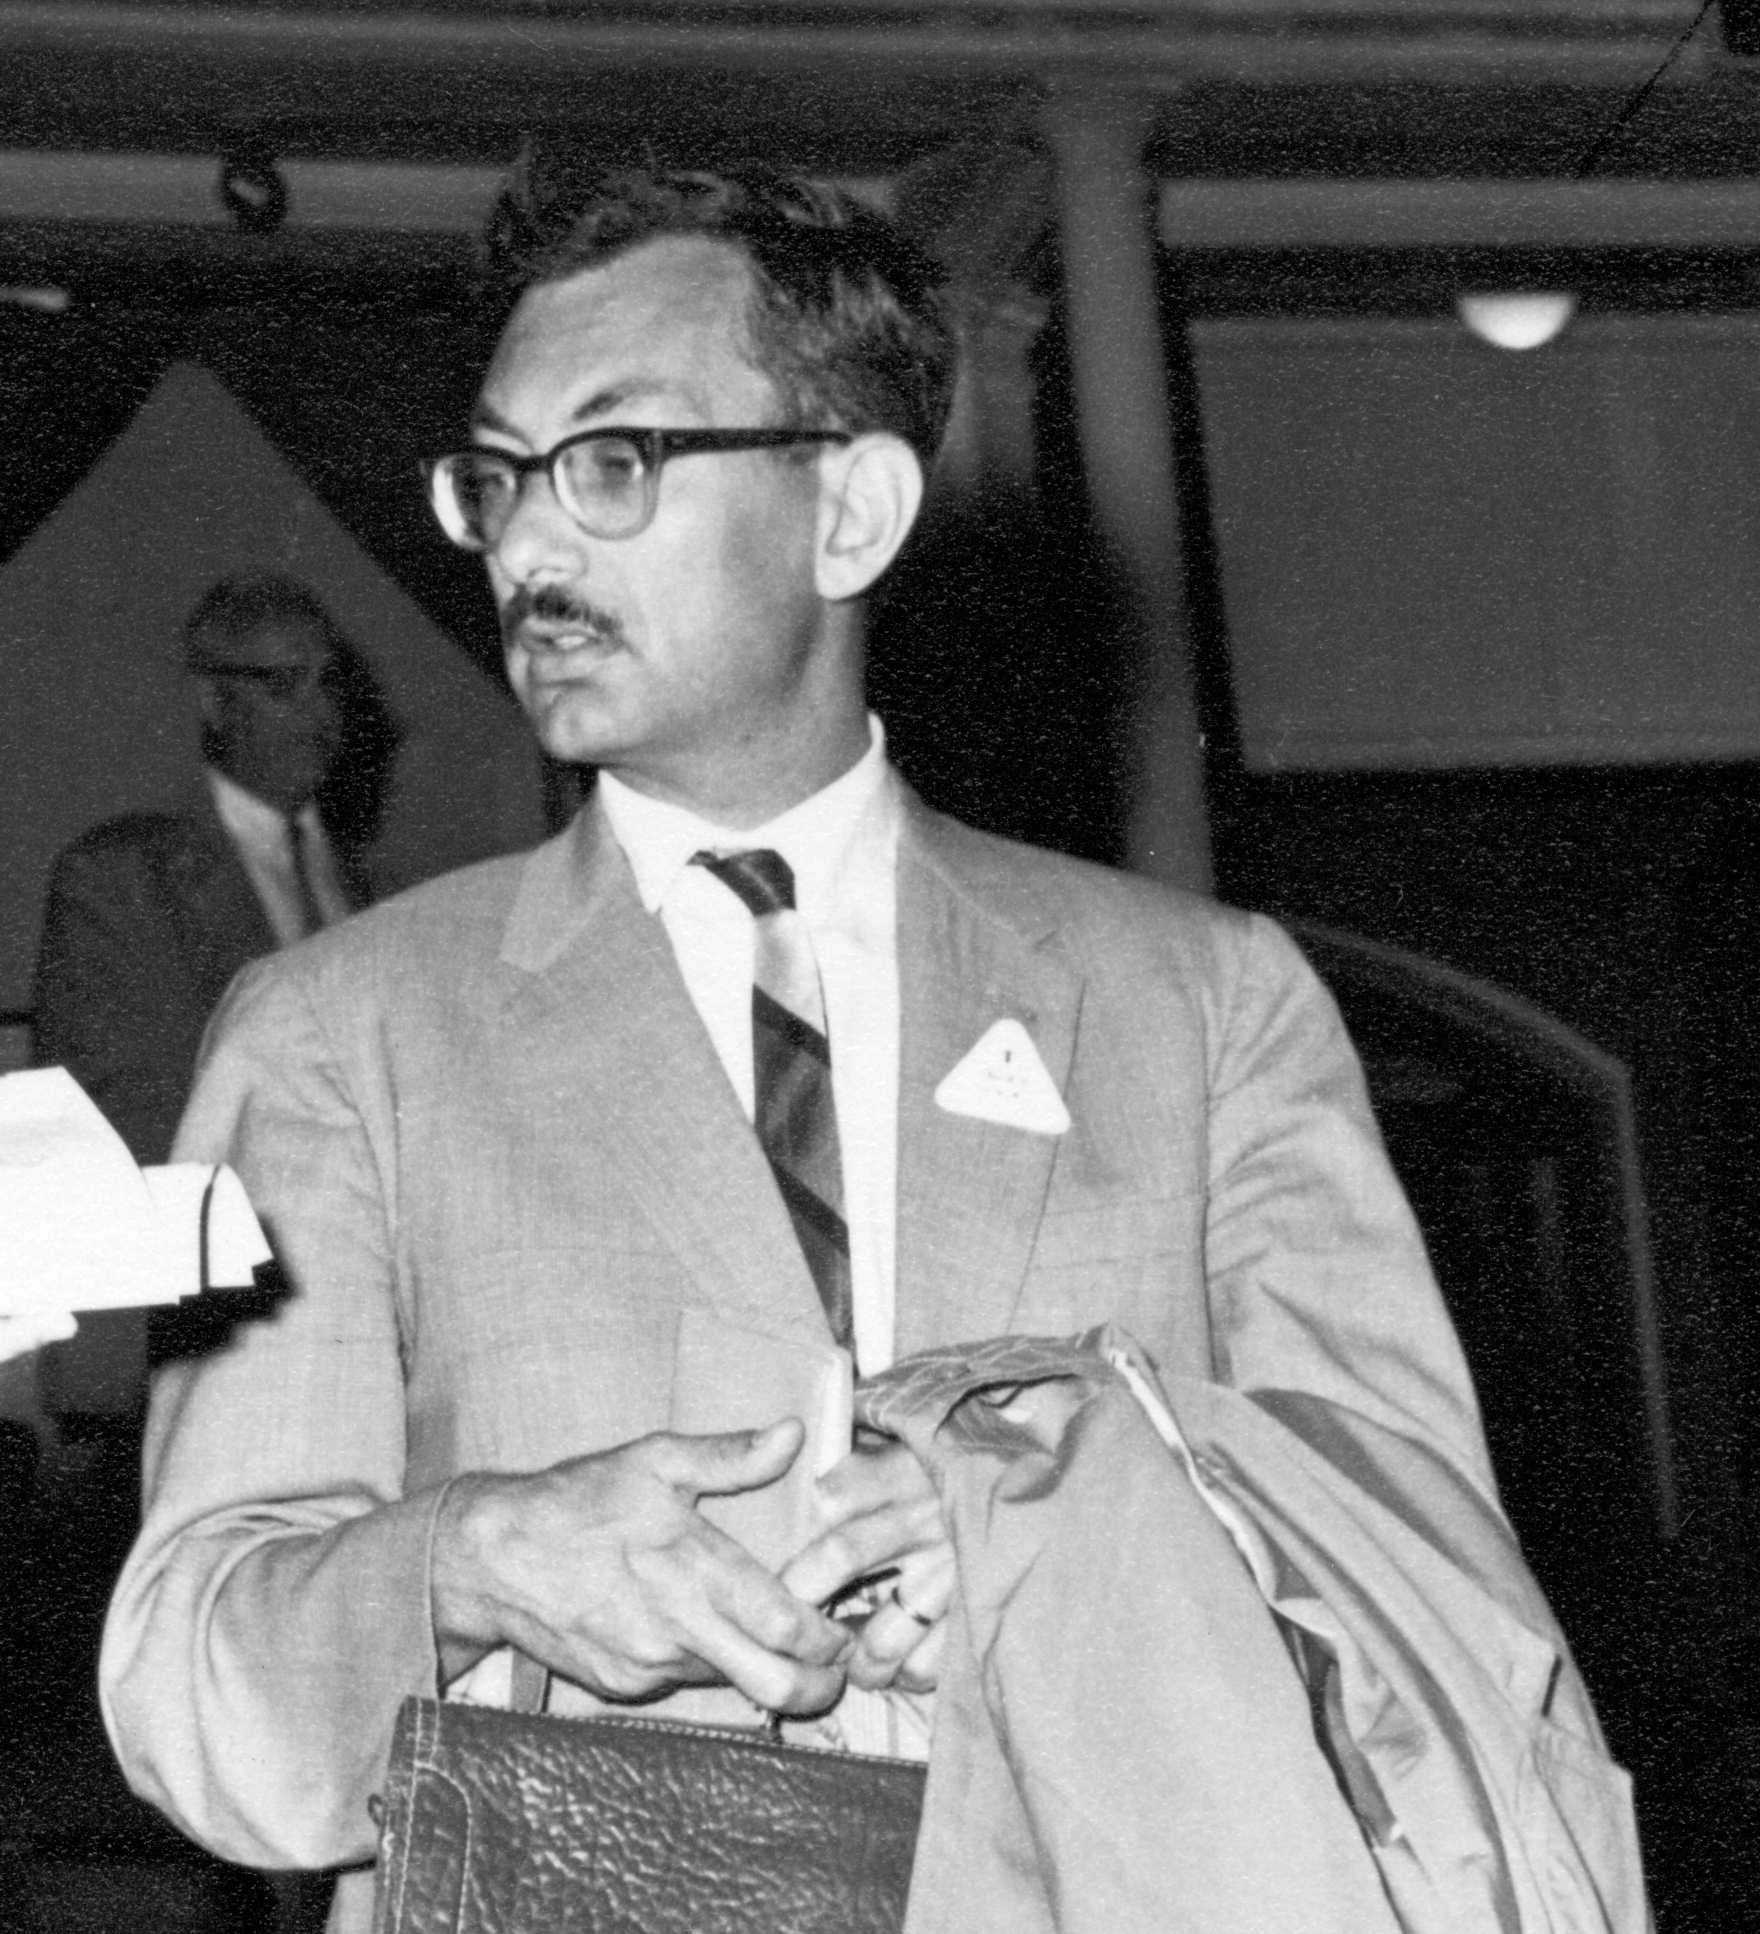
\includegraphics[height=1.9in]{rrs5.ps}
\end{tabular}
\end{center}
\bigskip

... as they were advocating phenetic classification.  Sokal did pioneering
investigations of
parsimony methods -- intending to show that they wouldn't work well!

\end{slide}

\begin{slide}[Replace]{The first numerical phylogeny, by Sokal and Michener 1957}

\begin{center}
\includegraphics[width=2.9in]{sokaltree.ps}
\end{center}

A tree of bees (Michener is the world's greatest bee systematist).
Michener was the one who wanted to interpret this as a phylogeny.  It was
inferred by a clustering method (not, as misstated in my book, by UPGMA).

\end{slide}

\begin{slide}[Replace]{Cavalli-Sforza and Edwards, 1963; Edwards, 1970}

\begin{center}
\begin{tabular}{r l}
\includegraphics[height=2.6in]{cavedwards3.ps} &
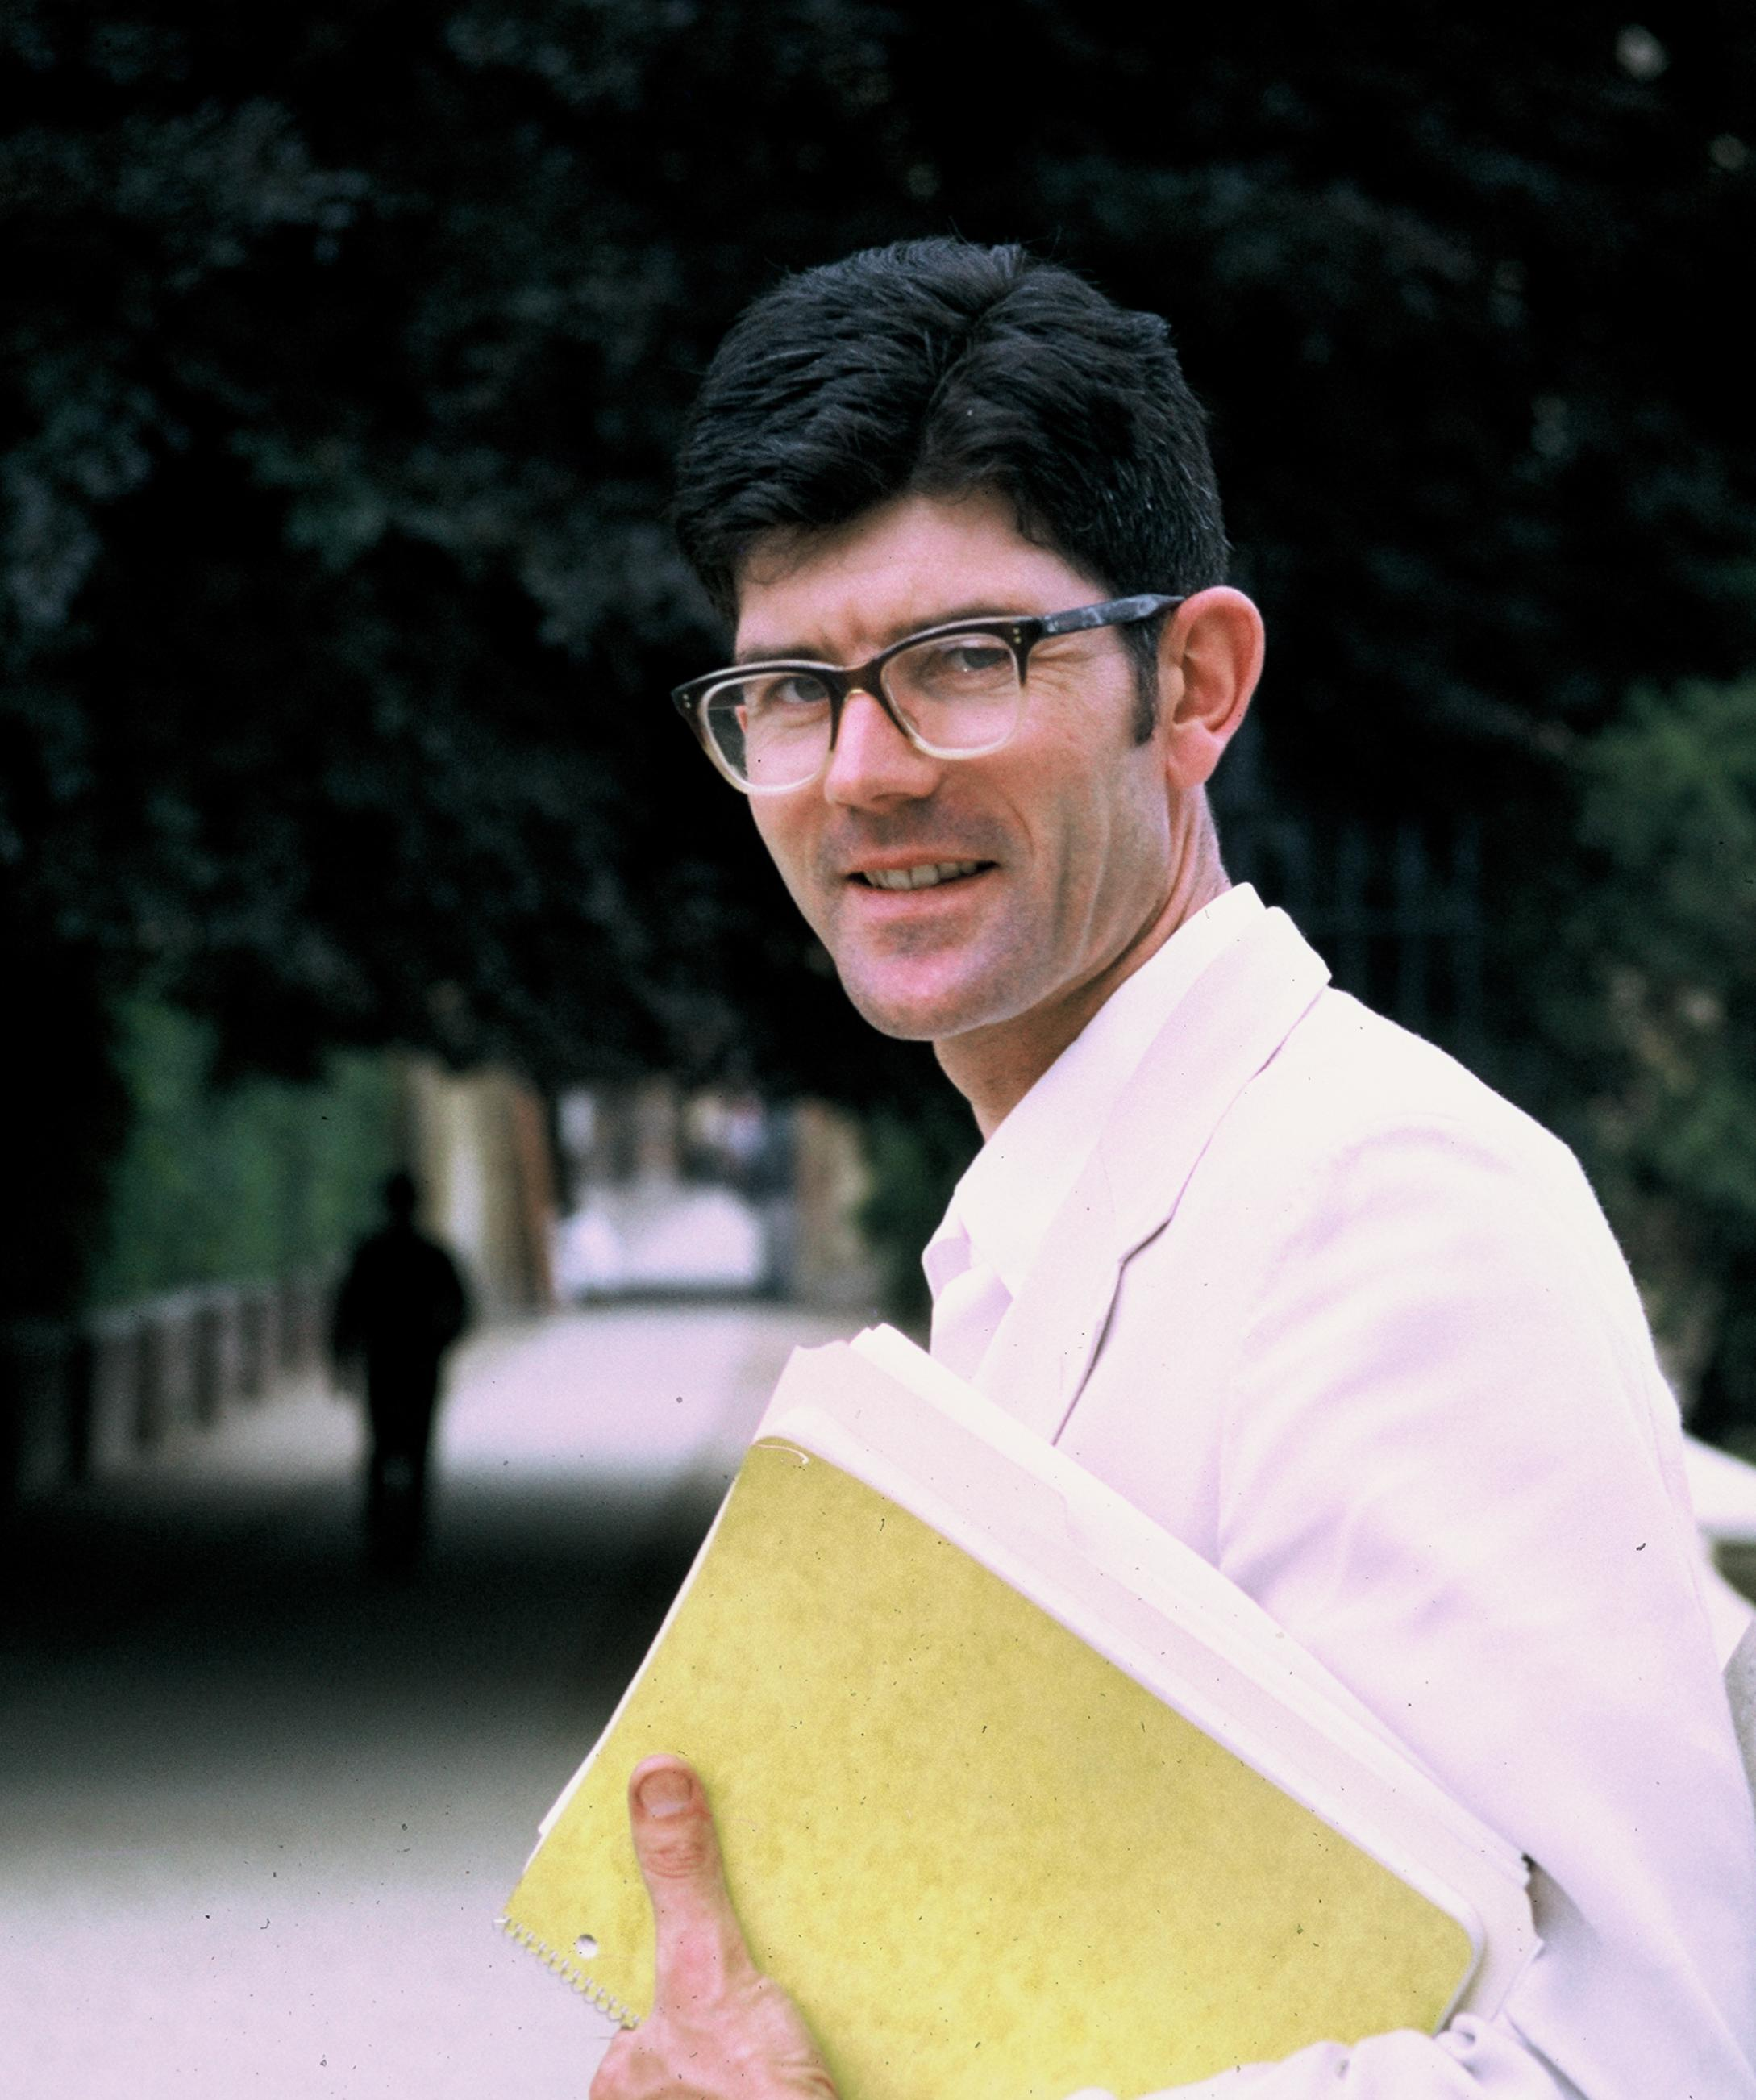
\includegraphics[height=2.6in]{edwards6.ps}
\end{tabular}
\end{center}

The picture on the left was taken by the famous population geneticist
Motoo Kimura when he and his family visited Pavia and were taken
on an excursion to a vineyard.

\end{slide}

\begin{slide}[Replace]{The first phylogeny by parsimony}

\begin{center}
\includegraphics[width=2.8in]{edwardstree3.ps}
\end{center}

Gene frequencies of blood group polymorphisms.  This is by minimum length in a space of gene frequencies.

\end{slide}

\begin{slide}[Replace]{That tree drawn out on a map}

\begin{center}
\includegraphics[width=4in]{edwardstree4.ps}
\end{center}
\bigskip

Note that the lineages from the Northwest Coast going down to Polynesia are
dependent on where on the map the splits are placed and that is somewhat
arbitrary.

\end{slide}

\begin{slide}[Replace]{Camin in the 1970s, one of the Caminalcules}

\begin{center}
\begin{tabular}{c c}
\includegraphics[height=2.4in]{camin3.ps} &
\includegraphics[height=2.4in]{caminalcule.ps}
\end{tabular}
\end{center}

Camin noticed (in 1965) that students who did the best job recovering the true
``phylogeny'' of the Caminalcules made the reconstruction which required the
fewest changes of state.

\end{slide}

\begin{slide}[Replace]{J. S. Farris and Arnold Kluge in the 1980s}

\begin{center}
\includegraphics[height=2in]{Farris3b.ps} \includegraphics[height=2in]{kluge.ps}
\end{center}

Further developments of parsimony methods, starting in 1969, advocacy of them
and of Hennig's
approach to classification during the 1970s and on.  Central in the rise (in
1980) of the Willi Hennig Society.

\end{slide}

\begin{slide}[Replace]{Margaret Dayhoff, 1966}

\begin{center}
\includegraphics[height=2.0in]{dayhoff2.ps}
\end{center}

{\ptsize{8}
\begin{itemize}
\setlength{\itemsep}{2pt}
\item A major pioneer of molecular databases (starting in 1965)
\item (With Richard Eck) made the first numerical phylogenies using molecular
data
\item Presented trees organized by gene families in the {\it Atlas of Protein
Sequences} (later the PIR database) in 1966.
\item Compiled the first empirical substitution rate matrices for amino acids,
intended to form the basis of a probabilistic model of protein evolution.
\end{itemize}
}

\end{slide}
\begin{slide}[Replace]{Walter Fitch, 1975}

\begin{center}
\includegraphics[height=2.0in]{Fitch3.ps}
\end{center}

Walter Fitch (1929-2011) :

{\ptsize{8} 
\begin{itemize}
\item The first major distance matrix method (1967) 
\item Developed algorithm (1971) that counts changes of state in DNA parsimony.
\item Introduced the terms and concepts of orthology and paralogy.
\item Co-founded the journal {\it Molecular Biology and Evolution} and the society SMBE.
\end{itemize}
}

\end{slide}

\begin{slide}[Replace]{Fitch and Margoliash's 1967 distance tree}

\begin{center}
\includegraphics[width=1.5in]{fitchtree.ps}\\
\includegraphics[width=1.5in]{fitchcaption.ps}\\
\end{center}

This is for globin sequences.  It is the first distance matrix method
published, if you don't count clustering methods.

\end{slide}

\begin{slide}[Replace]{Thomas Jukes and Charles Cantor, middle, in the 1990s}

\begin{center}
\includegraphics[height=2in]{jukes.ps} \includegraphics[height=2in]{cantor.ps}
\end{center}
\bigskip

But who are the two guys standing next to Charlie Cantor? ({\it Hint:} one has a Nobel
Prize, the other is a member of my own department).  Cantor later made important technical discoveries in genomics.  Jukes was
a nutritional biochemist who was the primary person responsible for insisting
that pregnant women get folic acid in their diet.

\end{slide}

\begin{slide}[Replace]{Jerzy Neyman: likelihood on molecular sequences}

\centerline{\includegraphics[height=2in]{neyman.ps}}
\bigskip

A major figure in mathematical statistics (he invented confidence intervals).
Statisticians don't know that he also
once worked on maximum likelihood inference of phylogenies from protein
sequences (usually he was known as a pointed critic of likelihood).

\end{slide}

\begin{slide}[Replace]{Willi Hennig (in 1972) and Walter Zimmermann (in 1959) }
\bigskip

\begin{center}
\begin{tabular}{c c c}
\includegraphics[height=1.5in]{Hennig3.ps} & \hspace{0.1in} &
\includegraphics[height=1.5in]{Zimmermann1959.ps} \\
 & & \\
Willi Hennig (1913-1976) & & Walter Zimmermann (1890-1980) \\
\end{tabular}
\end{center}
\bigskip

Zimmermann pioneered the method later advocated and made important by Hennig.
Hennig was the major advocate of a purely monophyletic classification system.

\end{slide}

\begin{slide}[Replace]{Hennig and conflict of characters}

W. Hennig (1966) says that in the case of homoplasy,

\begin{quote}
``it becomes necessary
to recheck the interpretation of [the] characters"
\end{quote}

He also says (1966, p. 121)

\begin{quote}
``the more certainly characters interpreted
as apomorphous (not characters in general) are present in a number of
different species, the better founded is the assumption that these species
form a morphological group."
\end{quote}

Farris, Kluge, and Eckardt (1970) argue that this should be translated as:

\begin{quote}
``the more characters certainly interpretable as apomorphous ..."
\end{quote}

\end{slide}

\begin{slide}[Replace]{Did Hennig invent parsimony?}

Farris (1983, p. 8):

\begin{quote}
I shall use the term in the sense I have already mentioned: most parsimonious
genealogical hypotheses are those that minimize requirements for ad hoc
hypotheses of homoplasy.  If minimizing ad hoc hypotheses is not the only
connotation of ``parsimony" in general useage, it is scarcely novel.  Both
Hennig (1966) and Wiley (1975) have advanced ideas closely related to my
useage.  Hennig defends phylogenetic analysis on the grounds of his
auxiliary principle, which states that homology should be presumed in the
absence of evidence to the contrary.  This amounts to the precept that
homoplasy ought not be postulated beyond necessity, that is to say
parsimony.
\end{quote}

\end{slide}

\begin{slide}[Replace]{Hennig's auxiliary principle}

Hennig discusses the case in which ``only one character can
certainly or with reasonable probability be interpreted as apomorphous."

Hennig (1966, p. 121):

\begin{quote}
In such cases it is impossible to decide whether the common character
is indeed synapomorphous or is to be interpreted as parallelism, homoiology,
or even as convergence.  I have therefore called it an ``auxiliary principle"
that the presence of apomorphous characters in different species ``is always
reason for suspecting kinship [i.e. that the species belong to a monophyletic
group], and that their origin by convergence should not be assumed a priori"
(Hennig 1953).  This was based on the conviction that ``phylogenetic
systematics would lose all the ground on which it stands" if the presence of
apomorphous characters in different species were considered first of all as
convergences (or parallelisms), with proof to the contrary required in
each case.
\end{quote}

This is usually considered to be a statement of parsimony.  Is it?

\end{slide}

\begin{slide}[Replace]{Farris and Kluge on Hennig and parsimony}

\begin{quote}
Unfortunately, AIV is not sufficiently detailed to allow us to select a
unique criterion for choosing a most preferable tree.  We know that trees on
which the monophyletic groups share many steps are preferable to trees on
which this is not so.  But AIV deals only with single monophyletic groups 
and does not tell us how to evaluate a tree consisting of several
monophyletic groups.  One widely used criterion -- parsimony -- could be used
to select trees.  This would be in accord with AIV, since on a most
parsimonious tree OTUs [tips] that share many states (this is {\it not} the
same as the OTUs' being {\it described} by many of the same {\it states})
are generally placed together.  We might argue that the parsimony criterion
selects a tree most in accord with AIV by ``averaging" in some sense the
preferability of all the monophyletic groups of the tree.  Other criteria,
however, may also agree with AIV.
\end{quote}

\begin{flushright}
Farris, Eckardt and Kluge, 1970
\end{flushright}

\end{slide}

\begin{slide}[Replace]{Philosophical frameworks: hypothetico-deductive}

Gaffney (1979, pp. 98-99)
\begin{quote}
In any case, in a hypothetico-deductive system, parsimony is not merely a
methodological convention, it is a direct corollary of the falsification
criterion for hypotheses (Popper, 1968a, pp. 144-145).  When we accept the
hypothetico-deductive system as a basis for phylogeny reconstruction, we
try to test a series of phylogenetic hypotheses in the manner indicated
above.  If all three of the three possible three-taxon statements are falsified at
least once, the least-rejected hypothesis remains as the preferred one,
not because of an arbitrary methodological rule, but because it best meets our
criterion of testability.  In order to accept an hypothesis that has been
successfully falsified one or more times, we must adopt an {\it ad hoc}
hypothesis for each falsification .... Therefore, in a system that seeks
to maximize vulnerability to criticism, the addition of {\it ad hoc}
hypotheses must be kept to a minimum to meet this criterion.
\end{quote}

\end{slide}

\begin{slide}[Replace]{more from Gaffney}

Gaffney (1979)
\begin{quote}
``the use of derived character distributions as articulated by
Hennig (1966) appears to fit the hypothetico-deductive model best."
\end{quote}

Gaffney (1979, p. 98)

\begin{quote}
``it seems to me that
parsimony, or Ockham's razor, is equivalent to `logic' or `reason' because
any method that does not follow the above principle would be incompatible
with any kind of predictive or causal system."
\end{quote}

\end{slide}

\begin{slide}[Replace]{Hypothetico-deductivists on falsification}

Eldredge and Cracraft (1980, p. 69) are careful to point out that

\begin{quote}
``Falsified" implies that
the hypotheses are proven false, but this is not the meaning we (or other
phylogenetic systematists) wish to convey.  It may be that the preferred
hypothesis will itself be ``rejected" by some synapomorphies.
\end{quote}

Wiley (1981, p. 111):

\begin{quote}
In other words, we have no external criterion to say that a particular
conflicting character is actually an invalid test.  Therefore, saying that
it is an invalid test
simply because it is unparsimonious is a statement that is, itself, an
ad hoc statement.  With no external criterion, we are forced to use parsimony
to minimize the total number of ad hoc hypotheses (Popper, 1968a: 145).
The result is that the most parsimonious of the various alternates is the
most highly corroborated and therefore preferred over the less parsimonious
alternates.
\end{quote}

\end{slide}

\begin{slide}[Replace]{Farris on hypothetico-deductivism}

Farris (1983, p. 8):

\begin{quote}
Wiley [(1975)] discusses parsimony in a Popperian context, characterizing
most parsimonious genealogies as those that are least falsified on available
evidence.  In his treatment, contradictory character distributions provide
putative falsifiers of  genealogies.  As I shall discuss below, any such
falsifier engenders a requirement for an ad hoc hypothesis of homoplasy
to defend the genealogy.  Wiley's concept is then equivalent to mine.
\end{quote}

\end{slide}

\begin{slide}[Replace]{Philosophical frameworks: Logical-parsimony}

Beatty and Fink (1979):

\begin{quote}
We can account for the necessity of parsimony (or some such consideration)
because evidence considerations alone are not sufficient.  But we have no
philosophical or logical argument with which to justify the use of
parsimony considerations -- a not surprising result, since this issue has
remained a philosophical dilemma for hundreds of years.
\end{quote}

This moves away from considering parsimony as justified by
hypothetico-deductive frameworks and invokes it as its own justification.

\end{slide}

\begin{slide}[Replace]{Kluge and Wolf on logical parsimony}

Kluge and Wolf (1993, p. 196):

\begin{quote}
Finally, we might imagine that some of the popularity of the aforementioned
methodological strategies and resampling techniques, and assumption of
independence in the context of taxonomic congruence and the cardinal rule of
Brooks and McLennan (1991), derives from the belief that phylogenetic
inference is hypothetico-deductive (e.g. Nelson and Platnick, 1984: 143-144),
or at least that it should be.  Even the uses to which some might put
cladograms, such as ``testing" adaptation (Coddington, 1988), are presented
as hypothetico-deductive.  But this ignores an alternative, that cladistics,
and its uses, may be an abductive enterprise (Sober, 1988).  We suggest that
the limits of phylogenetic systematics will be clarified considerably
when cladists understand how their knowledge claims are made (Rieppel, 1988;
Panchen, 1992).
\end{quote}

Again, moving away from hypothetico-deductivism.

\end{slide}

\begin{slide}[Replace]{Elliot Sober on falsification}

Sober (1988, p. 126):

\begin{quote}
Popper's philosophy of science is very little help here, because he has
little to say about {\it weak} falsification.  Popper, after all is a
hypothetico-{\it deductivist}.  For him, observational claims are deductive
consequences of the hypothesis under test .... Deductivism excludes
the possibility of probabilistic testing.  A theory that assigns probabilities
to various possible observational outcomes cannot be strongly falsified by
the occurrence of any of them.  This, I suggest, is the situation we confront
in testing phylogenetic hypotheses.  (AB)C is logically consistent with
all possible character distributions (polarized or not), and the same is
true of A(BC).  [Emphasis in the original]
\end{quote}

Sober sees Popper's hypothetico-deductive framework as ill-suited to
inference of phylogenies.

\end{slide}

\begin{slide}[Replace]{Philosophical foundations: Logical probability?}

\noindent
Popper's corroboration formula
\[
\mathsf{C(h, e, b) \ = \ \frac{p(e, hb) - p(e, b)}{p(e, hb) - p(eh, b) + p(e, b)}}
\]

\noindent
where\\
\begin{tabular}{l l l}
$\mathsf{b}$ & $\mathsf{=}$ & background knowledge \\
$\mathsf{h}$ & $\mathsf{=}$ & hypothesis \\
$\mathsf{e}$ & $\mathsf{=}$ & evidence  ($\mathsf{ = d},$  data?)
\end{tabular}

\[
\mathsf{C(h, e, b) \ = \ \frac{\Prob(d | h) - \Prob(d)}{\Prob(d | h) - \Prob(d \& h) + \Prob(d)}}
\]

This is used as a justification for parsimony, not actually as a
statistical method in spite of people like Kluge calling it ``logical
probability''.  Issue:  how to compute $\ \mathsf{\PROB(d)}\ $ and $\ \mathsf{\PROB(d \& h)}\ $ if you aren't a
Bayesian and can't weight by a prior on hypotheses?

\end{slide}

\begin{slide}[Replace]{Criticisms of statistical inference}

{\parindent=0in

Farris (1983, p.17):

\begin{quote}
The statistical approach to phylogenetic inference was wrong from the
start, for it rests on the idea that to study phylogeny at all, one must
first know in great detail how evolution has proceeded.
\end{quote}
\bigskip

Kluge (1997a)

\begin{quote}
``As an aside, the fact that the study of phylogeny is concerned with the
discovery of historical singularities means that calculus probability and
standard (Neyman-Pearson) statistics {\it cannot} apply to that historical
science ...."
\end{quote}
}

If, after tossing a coin multiple times, you lose the coin, does he think you
can't then analyze those data?

\end{slide}

\begin{slide}[Replace]{Positions on classification nowadays}

\begin{itemize}
\item \textcolor{purple}{Phylogenetic systematics.} ~ Willi Hennig advocated purely monophyletic
classification.  Now the (strongly) dominant approach.
\item \textcolor{purple}{Evolutionary systematics.} ~ Has almost faded away.  Its adherents were
reluctant to make it algorithmic.
\item \textcolor{purple}{Phenetics.} ~ Although Sokal and Sneath strongly influenced the field of
numerical clustering, their approach to biological classification has few
adherents.
\item \textcolor{purple}{IDMVM} ~ One person (me) takes the view that It Doesn't Matter Very Much,
as we use the phylogeny, and, given that, we never use the classification
system.  This is widely regarded as a marginal crackpot view [``A bizarre
thumb in the eye to systematists'' -- Michael Sanderson].
\end{itemize}

\end{slide}

\end{document}
